\documentclass[a4paper,11pt]{article}
\usepackage{amsmath,amsthm,amsfonts,amssymb,amscd,amstext,vmargin,graphics,graphicx,tabularx,multicol} 
\usepackage[francais]{babel}
\usepackage[utf8]{inputenc}  
\usepackage[T1]{fontenc} 
\usepackage{pstricks-add,tikz,tkz-tab,variations}
\usepackage[autolanguage,np]{numprint} 
\usepackage{color}
\usepackage{ulem}

\setmarginsrb{1.5cm}{0.5cm}{1cm}{0.5cm}{0cm}{0cm}{0cm}{0cm} %Gauche, haut, droite, haut
\newcounter{numexo}
\newcommand{\exo}[1]{\stepcounter{numexo}\noindent{\bf Exercice~\thenumexo} : \marginpar{\hfill /#1}}
\reversemarginpar


\newcounter{enumtabi}
\newcounter{enumtaba}
\newcommand{\q}{\stepcounter{enumtabi} \theenumtabi.  }
\newcommand{\qa}{\stepcounter{enumtaba} (\alph{enumtaba}) }
\newcommand{\initq}{\setcounter{enumtabi}{0}}
\newcommand{\initqa}{\setcounter{enumtaba}{0}}

\newcommand{\be}{\begin{enumerate}}
\newcommand{\ee}{\end{enumerate}}
\newcommand{\bi}{\begin{itemize}}
\newcommand{\ei}{\end{itemize}}
\newcommand{\bp}{\begin{pspicture*}}
\newcommand{\ep}{\end{pspicture*}}
\newcommand{\bt}{\begin{tabular}}
\newcommand{\et}{\end{tabular}}
\renewcommand{\tabularxcolumn}[1]{>{\centering}m{#1}} %(colonne m{} centrée, au lieu de p par défault) 
\newcommand{\tnl}{\tabularnewline}

\newcommand{\trait}{\noindent \rule{\linewidth}{0.2mm}}
\newcommand{\hs}[1]{\hspace{#1}}
\newcommand{\vs}[1]{\vspace{#1}}

\newcommand{\N}{\mathbb{N}}
\newcommand{\Z}{\mathbb{Z}}
\newcommand{\R}{\mathbb{R}}
\newcommand{\C}{\mathbb{C}}
\newcommand{\Dcal}{\mathcal{D}}
\newcommand{\Ccal}{\mathcal{C}}
\newcommand{\mc}{\mathcal}

\newcommand{\vect}[1]{\overrightarrow{#1}}
\newcommand{\ds}{\displaystyle}
\newcommand{\eq}{\quad \Leftrightarrow \quad}
\newcommand{\vecti}{\vec{\imath}}
\newcommand{\vectj}{\vec{\jmath}}
\newcommand{\Oij}{(O;\vec{\imath}, \vec{\jmath})}
\newcommand{\OIJ}{(O;I,J)}

\newcommand{\bmul}[1]{\begin{multicols}{#1}}
\newcommand{\emul}{\end{multicols}}

\newcommand{\reponse}[1][1]{%
\multido{}{#1}{\makebox[\linewidth]{\rule[0pt]{0pt}{20pt}\dotfill}
}}

\newcommand{\titre}[5] 
% #1: titre #2: haut gauche #3: bas gauche #4: haut droite #5: bas droite
{
\noindent #2 \hfill #4 \\
#3 \hfill #5

\vspace{-1.6cm}

\begin{center}\rule{6cm}{0.5mm}\end{center}
\vspace{0.2cm}
\begin{center}{\large{\textbf{#1}}}\end{center}
\begin{center}\rule{6cm}{0.5mm}\end{center}
}



\begin{document}
\pagestyle{empty}
\titre{Interrogation  : Bases de la géométrie}{Nom :}{Prénom :}{Classe}{Date}

\vspace*{0.5cm}
\begin{flushleft}
\begin{tabular}{|m{9.5cm}|m{1.25cm}|m{1.25cm}|m{1.25cm}|m{1.25cm}|m{1.25cm}|}
\hline 
\textbf{Compétences} & \begin{center}
\textbf{N.E.}
\end{center} & \begin{center}
\textbf{M.I.}
\end{center} & \begin{center}
\textbf{M.F.}
\end{center}  & \begin{center}
\textbf{M.S.}
\end{center} & \begin{center}
\textbf{T.B.M.}
\end{center} \\ 
\hline 
Je dois savoir utiliser un vocabulaire approprié &  &  & & &\\
\hline 
Je dois savoir définir et tracer un point, un segment, une droite et une demi-droite &  &  & & &\\
\hline
Je dois savoir lire et utiliser les symboles d'appartenance et de non-appartenance &  &  & & &\\ 
\hline

\end{tabular} 
\end{flushleft}

\textit{N.E = Non évalué ; M.I. = Maîtrise insuffisante ; M.F. = Maîtrise fragile ; M.S. = Maîtrise satisfaisante ; T.B.M. = Très bonne maîtrise}\\


\vspace*{0.5cm}


\exo{3} Questions de cours\\

\q Donner la définition d'une demi-droite.\\
\reponse[5]\\

\q Trouver les erreurs dans le tracé de la figure ci-dessous et \textbf{corriger-les}.
\begin{center}

\includegraphics[scale=0.8]{construction.eps} 
\end{center}

\q Donner les étapes de constructions de la figure ci-dessus.\\
\reponse[5]\\

\newpage

\vspace*{0.5cm}

\exo{1,5}

\bmul{2}


\noindent Tracer en vert le segment d'extrémités D et C. \\
Tracer en rouge la droite passant par les points A et C.\\
Tracer en bleu la demi-droite d'origine D passant par le point B.

\columnbreak


\includegraphics[scale=1.1]{exointerro1.eps} \\

\emul



\vspace*{0.5cm}

\exo{2} Indiquer le nom de la partie en gras du dessin.\\



\includegraphics[scale=0.85]{exointerro4.eps}   \hspace*{0.75cm} \includegraphics[scale=0.85]{exointerro5.eps} \\


\vspace*{0.75cm}

\exo{1.5} Repasser en couleur la partie demandée.\\


\includegraphics[scale=0.85]{exointerro6.eps}   \hspace*{0.75cm} \includegraphics[scale=0.85]{exointerro7.eps} \\

\vspace*{0.75cm}

\exo{2} \initq 
\bmul{2}

\includegraphics[scale=1]{exointerro8.eps} 

\columnbreak

\q Compléter avec les symboles $\in $ ou $\notin$.\\


\bmul{2}

B . . . [AH)\\

F  . . . (DE)\\

G . . . [FG] \\


\columnbreak
C . . . [AE]\\

H  . . . [BA)\\

A . . .  [HB)\\

\emul

\q Placer le point R tel que R $\in $ [BD) et R $\notin $ [FB).\\



\emul

\end{document}
